\documentclass[12pt,a4paper]{article}
\usepackage[titletoc]{appendix}
\usepackage{xeCJK}
\usepackage{amsmath}
\usepackage{array}
\usepackage{bm}
\usepackage{booktabs}
\usepackage{caption}
\usepackage{cite}
\usepackage{comment}
\usepackage{float}
\usepackage{fontspec} % xelatex限定
\usepackage{geometry}
\usepackage{graphicx}
\usepackage{indentfirst}
% \usepackage[utf8]{inputenc} % 非xelatex编译,显式指定文件编码为utf8
\usepackage{listings}
\usepackage{longtable}
\usepackage{mathtools}
\usepackage{multicol}
\usepackage{multirow}
\usepackage{supertabular}
\usepackage{subcaption}
\usepackage{tabu}
\usepackage{ulem}
\usepackage{url}
\usepackage{xcolor}
\usepackage{nccmath} % だが align* は nccmath が無くても使えるので敢えて両方書いた。
% \usepackage{CJKutf8}
% \usepackage{hyperref}

\geometry{a4paper,left=2.5cm,right=2.5cm,top=2.5cm,bottom=2.5cm}
\defaultCJKfontfeatures{Scale=1.2}
\linespread{1.5}

%% Define a new 'leo' style for the package that will use a smaller font.
\makeatletter
\def\url@leostyle{%
  \@ifundefined{selectfont}{\def\UrlFont{\sf}}{\def\UrlFont{\small\ttfamily}}}
\makeatother
\urlstyle{leo} % Now actually use the newly defined style.


\renewcommand{\contentsname}{\centering{目录}}
\renewcommand{\abstractname}{\large{摘要}}
\def\tablename{表}
\def\figurename{图}
\renewcommand{\thetable}{\thesection.\arabic{table}}
\renewcommand{\thefigure}{\thesection.\arabic{figure}}
\renewcommand{\multirowsetup}{\centering}
\renewcommand{\appendixname}{附录~\Alpha{section}}
\renewcommand{\refname}{参考文献}

\everymath{\displaystyle}
\bibliographystyle{plain}


\lstdefinestyle{BASH}{
    breaklines=true,                                     % 自动换行
    columns=fixed,
    extendedchars=true,                                  % lets you use non-ASCII characters; for 8-bits encodings only, does not work with UTF-8
    frame=shadowbox,                                     % 设置背景边框
    numbers=left,                                        % 在左侧显示行号
    numberstyle=\footnotesize\color{darkgray},           % 设定行号格式
    showstringspaces=false,                              % 不显示字符串中的空格
    tabsize=4,	                                         % 设置tab长度
}
\lstdefinestyle{tinyBASH}{
    breaklines=true,                                     % 自动换行
    basicstyle=\footnotesize\ttfamily,
    columns=fixed,
    extendedchars=true,                                  % lets you use non-ASCII characters; for 8-bits encodings only, does not work with UTF-8
    frame=shadowbox,                                     % 设置背景边框
    numbers=left,                                        % 在左侧显示行号
    numberstyle=\footnotesize\color{darkgray},           % 设定行号格式
    showstringspaces=false,                              % 不显示字符串中的空格
    tabsize=4,	                                         % 设置tab长度
}
\lstdefinestyle{Python}{
    breaklines=true,                                     % 自动换行
    captionpos=b,                                        % sets the caption-position to bottom
    columns=fixed,
    commentstyle=\it\color[RGB]{0,96,96},                % 设置代码注释的格式
    % extendedchars=true,                                  % lets you use non-ASCII characters; for 8-bits encodings only, does not work with UTF-8
    frame=shadowbox,                                     % 设置背景边框
    keywordstyle=\bfseries\color[RGB]{40,40,255},        % 设定关键字颜色
    language=Python,                                     % 设置语言
    numbers=left,                                        % 在左侧显示行号
    numberstyle=\footnotesize\color{darkgray},           % 设定行号格式
    stringstyle=\rmfamily\slshape\color[RGB]{128,0,0},   % 设置字符串格式
    tabsize=4,	                                         % 设置tab长度
}

\lstdefinestyle{CPP}{
    %backgroundcolor=\color[RGB]{245,245,244},           % 设定背景颜色
    breaklines=true,                                     % 自动换行
    captionpos=b,                                        % sets the caption-position to bottom
    columns=fixed,
    commentstyle=\it\color[RGB]{0,96,96},                % 设置代码注释的格式
    extendedchars=true,                                  % lets you use non-ASCII characters; for 8-bits encodings only, does not work with UTF-8
    frame=shadowbox,                                     % 设置背景边框
    keywordstyle=\bfseries\color[RGB]{40,40,255},        % 设定关键字颜色
    language=c++,                                        % 设置语言
    numbers=left,                                        % 在左侧显示行号
    numberstyle=\footnotesize\color{darkgray},           % 设定行号格式
    showstringspaces=false,                              % 不显示字符串中的空格
    stringstyle=\rmfamily\slshape\color[RGB]{128,0,0},   % 设置字符串格式
    tabsize=4,	                                         % 设置tab长度
    title=\lstname,                                      % show the filename of files included with \lstinputlisting; also try caption instead of title
    morekeywords={alignas,continute,friend,register,true,alignof,decltype,goto,
        reinterpret_cast,try,asm,defult,if,return,typedef,auto,delete,inline,short,
        typeid,bool,do,int,signed,typename,break,double,long,sizeof,union,case,
        dynamic_cast,mutable,static,unsigned,catch,else,namespace,static_assert,using,
        char,enum,new,static_cast,virtual,char16_t,char32_t,explict,noexcept,struct,
        void,export,nullptr,switch,volatile,class,extern,operator,template,wchar_t,
        const,false,private,this,while,constexpr,float,protected,thread_local,
        const_cast,for,public,throw,std},
    emph={map,set,multimap,multiset,unordered_map,unordered_set,
        unordered_multiset,unordered_multimap,vector,string,list,deque,
        array,stack,forwared_list,iostream,memory,shared_ptr,unique_ptr,
        random,bitset,ostream,istream,cout,cin,endl,move,default_random_engine,
        uniform_int_distribution,iterator,algorithm,functional,bing,numeric},
}

\lstdefinestyle{QT}{
    %backgroundcolor=\color[RGB]{245,245,244},           % 设定背景颜色
    breaklines=true,                                     % 自动换行
    captionpos=b,                                        % sets the caption-position to bottom
    columns=fixed,
    commentstyle=\it\color[RGB]{0,96,96},                % 设置代码注释的格式
    extendedchars=true,                                  % lets you use non-ASCII characters; for 8-bits encodings only, does not work with UTF-8
    frame=shadowbox,                                     % 设置背景边框
    keywordstyle=\bfseries\color[RGB]{40,40,255},        % 设定关键字颜色
    language=c++,                                        % 设置语言
    numbers=left,                                        % 在左侧显示行号
    numberstyle=\footnotesize\color{darkgray},           % 设定行号格式
    stringstyle=\rmfamily\slshape\color[RGB]{128,0,0},   % 设置字符串格式
    showstringspaces=false,                              % 不显示字符串中的空格
    tabsize=4,	                                         % 设置tab长度
    title=\lstname,                                      % show the filename of files included with \lstinputlisting; also try caption instead of title
    morekeywords={alignas,continute,friend,register,true,alignof,decltype,goto,
        reinterpret_cast,try,asm,defult,if,return,typedef,auto,delete,inline,short,
        typeid,bool,do,int,signed,typename,break,double,long,sizeof,union,case,
        dynamic_cast,mutable,static,unsigned,catch,else,namespace,static_assert,using,
        char,enum,new,static_cast,virtual,char16_t,char32_t,explict,noexcept,struct,
        void,export,nullptr,switch,volatile,class,extern,operator,template,wchar_t,
        const,false,private,this,while,constexpr,float,protected,thread_local,
        const_cast,for,public,throw,std,bind,function,
        Q_OBJECT,QDialog,QUdpSocket,QTcpSocket,QHostAddress,QNetworkDatagram,QTcpServer,
        QByteArray,QString,QStringList,QList,QSet,QMap,
        quint,qint64,uintptr_t,
        connect,signals,slots,SIGNAL,SLOT},
    emph={map,set,multimap,multiset,unordered_map,unordered_set,
        unordered_multiset,unordered_multimap,vector,string,list,deque,
        array,stack,forwared_list,iostream,memory,shared_ptr,unique_ptr,
        random,bitset,ostream,istream,cout,cin,endl,move,default_random_engine,
        uniform_int_distribution,iterator,algorithm,functional,bing,numeric},
}

\lstdefinestyle{MASM}{
    breaklines=true,                                     % 自动换行
    captionpos=b,                                        % sets the caption-position to bottom
    columns=fixed,
    commentstyle=\it\color[RGB]{0,96,96},                % 设置代码注释的格式
    extendedchars=true,                                  % lets you use non-ASCII characters; for 8-bits encodings only, does not work with UTF-8    
    frame=shadowbox,                                     % 设置背景边框
    keywordstyle=\bfseries\color[RGB]{40,40,255},        % 设定关键字颜色
    language=[x86masm]Assembler,                         % 设置语言
    numbers=left,                                        % 在左侧显示行号
    numberstyle=\footnotesize\color{darkgray},           % 设定行号格式
    stringstyle=\rmfamily\slshape\color[RGB]{128,0,0},   % 设置字符串格式
    showstringspaces=false,                              % 不显示字符串中的空格
    tabsize=4,	                                         % 设置tab长度
    title=\lstname,                                      % show the filename of files included with \lstinputlisting; also try caption instead of title
    morekeywords={CDQE,CQO,CMPSQ,CMPXCHG16B,JRCXZ,LODSQ,MOVSXD, % 
        POPFQ,PUSHFQ,SCASQ,STOSQ,IRETQ,RDTSCP,SWAPGS, % 
        .code,.def,.file,.type,.ended,.scl,.section,.ascii,.text,.globl,.ident,.rodata,
        .sch_proc,.sch_pushreg,.sch_setframe,.sch_stackalloc,.sch_endprologue,.sch_endproc,
        pushq,popq,movq,movl,addq,subq,leaq,invoke,start,addr,
        rax,rdx,rcx,rbx,rsi,rdi,rip,rsp,rbp, % 
        r8,r8d,r8w,r8b,r9,r9d,r9w,r9b, % 
        r10,r10d,r10w,r10b,r11,r11d,r11w,r11b, % 
        r12,r12d,r12w,r12b,r13,r13d,r13w,r13b, % 
        r14,r14d,r14w,r14b,r15,r15d,r15w,r15b}
}
\newcommand{\includecode}[2][c]{\lstinputlisting[caption=#2, escapechar=, style=#1]{#2}}



% \setcounter{table}{0}
% \setcounter{figure}{0}

% \lstinputlisting[style=CPP]{src/main.cpp}

% \begin{figure}[H]
%     \centering
%     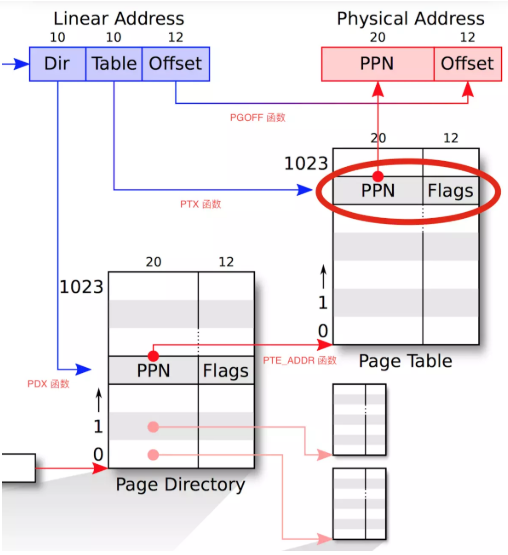
\includegraphics[width = .75\linewidth]{img/1.png}
%     \caption{预处理结果(部分)}
%     \label{fig::figure2}
% \end{figure}


% 结果如表\ref{tab::table2}:
% \begin{table}[htbp]
%     \begin{center}
%         \begin{tabular}{c c c}
%             \toprule
%             优化等级 & 二进制文件大小(Byte) &  执行时间(s)\\
%             \midrule
%             不优化 & 13992 & 36.090 \\
%             O1 & 13344 & 10.562\\
%             O2 & 13344 & 9.925\\
%             Os & 13344 & 8.899\\
%             O3 & 13344 & 8.350\\
%             Ofast & 14800 & 8.094\\
%             \bottomrule
%         \end{tabular}
%         \caption{各等级优化测试结果}\label{tab::table2}
%     \end{center}
% \end{table}

% \begin{equation}
%     \begin{split}
%         id     & \rightarrow char\ |\ id\ digit\ |\ id\ char \\
%         digit  & \rightarrow 0\ |\ 1\ |\ 2\ |\ 3\ |\ 4\ |\ 5\ |\ 6\ |\ 7\ |\ 8\ |\ 9 \\
%         char   & \rightarrow \_\ |\ letter \\
%         letter & \rightarrow A\ |\ B\ |\ ...\ |\ Z\ |\ a\ |\ b\ |\ ...\ |\ z \\
%     \end{split}
% \end{equation}

\begin{document}

\title{Lab 4:  Preemptive Multitasking}
\author{\ }

\maketitle

\begin{abstract}
    \setlength{\parindent}{2em}
    本次实验取自MIT\ 6.828\ Lab4,实现在同时运行的多个用户进程中实现抢占式多任务处理,实验共分为三个部分。

    在第一部分,为 JOS 系统添加多处理器支持,实现轮转调度,并在系统调用中添加一些基础进程管理方法(例如,创建、销毁进程,以及分配和映射内存)。
    
    在第二部分,实现类 Unix 的 fork() 方法,以允许用户进程创造自身的拷贝。
    
    在第三部分,为 JOS 提供进程间通信支持,允许不同的用户进程显式地彼此交流和同步,并实现硬件时钟中断和抢占。

    \textbf{关键词:JOS、抢占式多任务处理、轮转调度、系统调用、进程间通信}
\end{abstract}

\section{作业一}

修改你在 kern/pmap.c 中实现过的 page\_init() 以避免将 MPENTRY\_PADDR 加入到 free list 中,
以使得我们可以安全地将 AP 的引导代码拷贝于这个物理地址并运行。

\begin{lstlisting}[style=CPP]
pages[0].pp_ref = 1;
size_t size_ioh = 96;
size_t size_ext = ((uint32_t)boot_alloc(0) - KERNBASE) / PGSIZE;
size_t i, j = npages_basemem + size_ioh + size_ext, mpp = MPENTRY_PADDR / PGSIZE;
for (i = 1; i < npages; i++) {
    if (i == mpp || (i >= npages_basemem && i < j)) {
        //在不可用区域里加上MPENTRY_PADDR所在处
        pages[i].pp_ref = 1;//标记为不可用
        continue;
    }
    pages[i].pp_ref = 0;//标记为可用
    pages[i].pp_link = page_free_list;
    page_free_list = &pages[i];
}
\end{lstlisting}

\section{问题一}

逐行比较 kern/mpentry.S 和 boot/boot.S。牢记 kern/mpentry.S 和其他内核代码一样也是被编译和链接在 KERNBASE 之上运行的。
那么,MPBOOTPHYS 这个宏定义的目的是什么呢?为什么它在 kern/mpentry.S 中是必要的,但在 boot/boot.S 却不用?

因为mpentry.S的代码都在kernbase上,所以实模式是没办法直接寻址的,
这时候需要MPBOOTPHYS起一个地址转换的作用,而boot.S就被加载在实模式可寻址的低地址,所以不需要地址转换。

\section{作业二}

修改位于 kern/pmap.c 中的 mem\_init\_mp(),将每个CPU堆栈映射在 KSTACKTOP 开始的区域,就像 inc/memlayout.h 中描述的那样。
每个堆栈的大小都是 KSTKSIZE 字节,加上 KSTKGAP 字节没有被映射的守护页。

\begin{lstlisting}[style=CPP]
uintptr_t kstacktop_i;
for (int i = 0; i < NCPU; i++) {
    kstacktop_i = KSTACKTOP - i * (KSTKSIZE + KSTKGAP);
    boot_map_region(kern_pgdir, kstacktop_i - KSTKSIZE, KSTKSIZE, PADDR(percpu_kstacks[i]), PTE_W);
    //参数:目录,虚拟起始地址,大小,物理地址,权限
}
\end{lstlisting}

对于NCPU个栈区域,从KSTACKTOP开始向低地址延伸,每个区域大小为KSTLSIZE,栈区域之间有KSTKGAP大小的间隔,依次标记好位置后初始化。
用于遍历的临时变量从栈顶开始向下挪移,每次挪移堆栈大小+堆栈间隔)的长度。每次挪移对经过的堆栈进行映射。

\section{作业三}

需要做的工作是修改trap\_init\_percpu()函数使得它可以完成对每个CPU的初始化,具体来说就是将全局变量改成每个CPU的变量,新旧代码对比如下:

\begin{lstlisting}[style=CPP]
void
trap_init_percpu(void) {
    int cpu_id = thiscpu->cpu_id;
    struct Taskstate *this_ts = &thiscpu->cpu_ts;        
    
    // Setup a TSS so that we get the right stack
    // when we trap to the kernel.

    /*ts.ts_esp0 = KSTACKTOP;
    ts.ts_ss0 = GD_KD;*/

    this_ts->ts_esp0 = KSTACKTOP - cpu_id * (KSTKSIZE + KSTKGAP);
    this_ts->ts_ss0 = GD_KD;

    // Initialize the TSS slot of the gdt.

    /*gdt[GD_TSS0 >> 3] = SEG16(STS_T32A, (uint32_t) (&ts),sizeof(struct Taskstate) - 1, 0);
    gdt[GD_TSS0 >> 3].sd_s = 0;*/

    gdt[(GD_TSS0 >> 3) + cpu_id] = SEG16(STS_T32A, (uint32_t) (this_ts),sizeof(struct Taskstate) - 1, 0); 
    gdt[(GD_TSS0 >> 3) + cpu_id].sd_s = 0;

    // Load the TSS selector (like other segment selectors, the
    // bottom three bits are special; we leave them 0)

    //ltr(GD_TSS0);
    ltr(GD_TSS0 + (cpu_id << 3));

    // Load the IDT
    lidt(&idt_pd);
}
\end{lstlisting}

\section{作业四}
Apply the big kernel lock as described above, by calling lock\_kernel() andunlock\_kernel() at the proper locations.

大内核锁的实现:
\begin{lstlisting}[style=CPP]
void
spin_lock(struct spinlock* lk)
{
#ifdef DEBUG_SPINLOCK
    if (holding(lk))
        panic("CPU %d cannot acquire %s: already holding", cpunum(), lk->name);
#endif

    // The xchg is atomic.
    // It also serializes, so that reads after acquire are not
    // reordered before it. 
    // 关键代码,体现了循环等待的思想
    while (xchg(&lk->locked, 1) != 0)
        asm volatile ("pause");

    // Record info about lock acquisition for debugging.
#ifdef DEBUG_SPINLOCK
    lk->cpu = thiscpu;
    get_caller_pcs(lk->pcs);
#endif
}
\end{lstlisting}

其中,在 inc/x86.h 中可以找到 xchg() 函数的实现,使用它而不是用简单的 if 和赋值 是因为它是一个原子性的操作。
\begin{lstlisting}[style=CPP]
static inline uint32_t
xchg(volatile uint32_t* addr, uint32_t newval)
{
    uint32_t result;

    // The + in "+m" denotes a read-modify-write operand.
    asm volatile("lock; xchgl %0, %1"
        : "+m" (*addr), "=a" (result) // 输出
        : "1" (newval)                // 输入
        : "cc");
    return result;
}
\end{lstlisting}

这是一段内联汇编。lock 确保了操作的原子性,其意义是将 addr 存储的值与 newval 交换,并返回 addr 中原本的值。
于是,如果最初 locked = 0,即未加锁,就能跳出这个 while循环。否则就会利用 pause 命令自旋等待。
确保了当一个 CPU 获得了 BKL,其他 CPU 如果要获得就只能自旋等待。

在这几处加大内核锁为了避免多个 CPU 同时运行内核代码,保证独立性。由于分页机制的存在,内核以及每个用户进程都有自己的独立空间。
而多进程并发的时候,如果两个进程同时陷入内核态,就无法保证独立性了。例如内核中有某个全局变量 A,cpu1 让 A=1,而后 cpu2 却让 A=2,显然会互相影响。
为了使系统尽快支持 SMP,直接在内核入口加大内核锁锁,保证其独立性。

其流程大致为:

BPS 启动 AP 前,获取内核锁,所以 AP 会在 mp\_main 执行调度之前阻塞,在启动完 AP 后,BPS 执行调度,
运行第一个进程,env\_run() 函数中会释放内核锁,这样一来,其中一个 AP 就可以开始执行调度,运行其他进程。

\begin{lstlisting}[style=CPP]
// i386_init()
// Your code here:
lock_kernel();
boot_aps();
\end{lstlisting}

在唤醒其他 CPU 前需要 lock ,防止唤醒的 CPU 启动进程。
\begin{lstlisting}[style=CPP]
// mp_main()
// Your code here:
lock_kernel();
sched_yield();
\end{lstlisting}

初始化 AP 后,在调度之前需要 lock,防止其他 CPU 干扰进程的选择。
\begin{lstlisting}[style=CPP]
// trap()
// LAB 4: Your code here.
lock_kernel();
assert(curenv);
\end{lstlisting}

用户态引发中断陷入内核态时,需要 lock。
\begin{lstlisting}[style=CPP]
// env_run()
lcr3(PADDR(e->env_pgdir));
unlock_kernel();
env_pop_tf(&(e->env_tf));
\end{lstlisting}

离开内核态之前,需要 unlock 。

BPS 启动 AP 前,获取内核锁,所以 AP 会在 mp\_main 执行调度之前阻塞,在启动完 AP 后,BPS 执行调度,
运行第一个进程,之后释放内核锁,这样一来,其中一个 AP 就可以开始执行调度,若有的话运行进程。

\section{问题二}

It seems that using the big kernel lock guarantees that only one CPU can run the kernel code at a time. 
Why do we still need separate kernel stacks for each CPU? 
Describe a scenario in which using a shared kernel stack will go wrong, even with the protection of the big kernel lock.

如果内核栈中留下不同 CPU 之后需要使用的数据,可能会造成混乱。

例如在某进程即将陷入内核态的时候(尚未获得锁),系统在 trap() 函数之前已经在 trapentry.S 中对内核栈进行了操作,压入了寄存器信息。
如果共用一个内核栈,那显然会导致信息错误。

\section{作业五}

按照题目的要求在sched\_yield()函数实现轮转调度。具体实现方法是如果存在上一个running environment,
就从它开始,否则从头开始搜索envs数组,找到一个runnable的environment并进入。
如果没有其他environment而之前有一个正在运行的则继续执行它。其他情况执行cpuhalt代码如下:

\begin{lstlisting}[style=CPP]
void
sched_yield(void) {
    struct Env *idle;
    int i, k, envidx;

    if (curenv)
        envidx = ENVX(curenv->env_id);
    else
        envidx = 0;

    for (i = 0; i < NENV; ++i) {
        k = (envidx + i) % NENV;
        if (envs[k].env_status == ENV_RUNNABLE)
            env_run(&envs[k]);
    }
    if (curenv && curenv->env_status == ENV_RUNNING)
        env_run(curenv);

    // sched_halt never returns
    sched_halt();
}
\end{lstlisting}

还有,在syscall.c里补充相应的系统调用:

\begin{lstlisting}[style=CPP]
static void
sys_yield(void) {
   sched_yield();
}

int32_t
syscall(uint32_t syscallno, uint32_t a1, uint32_t a2, uint32_t a3, uint32_t a4, uint32_t a5) {
    ......
    case SYS_yield:
        sys_yield();
        return 0;
    ......
}
\end{lstlisting}

\section{问题三}

    在你实现的 env\_run() 中你应当调用了 lcr3()。在调用 lcr3() 之前和之后,你的代码应当都在引用 变量 e,
    就是 env\_run() 所需要的参数。 在装载 \%cr3 寄存器之后, MMU 使用的地址上下文立刻发生改变,
    但是处在之前地址上下文的虚拟地址(比如说e)却还能够正常工作,为什么 e 在地址切换前后都可以被正确地解引用呢?

    在env.c的env\_settup\_vm()中:

    \begin{lstlisting}[style=CPP]
e->env_pgdir = (pde_t *)page2kva(p);
p->pp_ref += 1;
memcpy(e->env_pgdir, kern_pgdir, PGSIZE);

// UVPT maps the env's own page table read-only.
// Permissions: kernel R, user R
e->env_pgdir[PDX(UVPT)] = PADDR(e->env_pgdir) | PTE_P | PTE_U;

return 0;
    \end{lstlisting}

    在env\_setup\_vm()中,注释说所有环境的虚拟地址空间从UTOP到UVPT都是相同的,内核的地址空间也是相同的。
    无论地址空间是什么,e的虚拟地址总是相同的。例如上述代码直接以内核的页目录作为模版进行复制,
    两个页目录的 e 地址映射到同一物理地址,e 在地址切换前后都可以被正确地解引用。

\section{作业六}

    作业6要求在 kern/syscall.c 中实现用于创建进程的系统调用,使得用户进程也可以创建和启动其他新的用户进程。
    其中系统调用包括sys\_exofork、sys\_env\_set\_status、sys\_page\_alloc()、sys\_page\_map()和sys\_page\_unmap()。
    具体实现过程如下:

    user/dumbfork.c 中提供的一种Unix 样式的 fork(),其duppage() 函数如下:
    \begin{lstlisting}[style=CPP]
void
duppage(envid_t dstenv, void *addr) {
int r;

// This is NOT what you should do in your fork.
if ((r = sys_page_alloc(dstenv, addr, PTE_P|PTE_U|PTE_W)) < 0)
    panic("sys_page_alloc: %e", r);
    
if ((r = sys_page_map(dstenv, addr, 0, UTEMP, PTE_P|PTE_U|PTE_W)) < 0)
    panic("sys_page_map: %e", r);
    
memmove(UTEMP, addr, PGSIZE);
if ((r = sys_page_unmap(0, UTEMP)) < 0)
    panic("sys_page_unmap: %e", r);
}
    \end{lstlisting}

    dumbfork()首先通过 sys\_exofork() 系统调用创建一个新的空白进程。

    然后通过duppage拷贝父进程的地址空间到子进程中。用户进程地址空间开始位置是UTEXT(0x00800000) ,结束位置是 end。
    其中duppage是一页页拷贝的,它将父进程的addr开始的一页物理内存内容拷贝到子进程dstenv的对应的页中。

    最后完成父进程到子进程内存数据的拷贝。先通过sys\_page\_alloc为子进程addr开始的一页内容分配一个物理页并完成映射,
    此时,分配的物理页还是空的,没有数据。然后通过 sys\_page\_map 将子进程va开始的这分配好的物理页映射到
    父进程的UTEMP地址处(0x00400000),使得在父进程中可以访问到子进程新分配的物理页。
    接下来,通过memmove函数将父进程addr处的一页数据拷贝到了UTEMP中,即将父进程的addr处的一页内存数据拷贝到
    子进程的addr对应的那页内存完成数据的复制(UTEMP已经映射到了子进程的那页内存)。
    最后通过 sys\_page\_unmap 取消父进程在UTEMP的映射以下次使用,同时预防父进程误操作到子进程的内存数据。

    \subsection{sys\_exofork()}
    sys\_exofork()创建一个用户地址空间没有内存映射,也不可以运行,几乎完全空白的新进程。

    使用env\_alloc()创建新环境。将状态设置为ENV\_NOT\_RUNNABLE,从当前环境中复制寄存器集,进行调整后使sys\_exofork看起来返回0。
    如果没有可用的空闲环境,返回-E\_NO\_FREE\_ENV,内存耗尽返回-E\_NO\_MEM。

    \begin{lstlisting}[style=CPP]
static envid_t
sys_exofork(void) {
    // LAB 4: Your code here.
    // panic("sys_exofork not implemented");
    struct Env *e;
    int err = env_alloc(&e, curenv->env_id);
    if (err < 0) 
        return err;

    e->env_status = ENV_NOT_RUNNABLE;
    e->env_tf = curenv->env_tf;
    e->env_tf.tf_regs.reg_eax = 0;

    return e->env_id;
}
    \end{lstlisting}

    \subsection{sys\_env\_set\_status()}
    sys\_env\_set\_status()可以将一个进程的状态设置为 ENV\_RUNNABLE 或 ENV\_NOT\_RUNNABLE。
    通常用来在新创建的进程的地址空间和寄存器状态已经初始化完毕后将它标记为就绪状态。

    使用kern/ Env. c中的'envid2env'函数将一个envid转换成一个结构Env。
    并将envid2env的第三个参数设置为1,用于检查当前环境是否具有设置envid状态的权限。
    成功返回0,错误返回< 0。-E\_BAD\_ENV代表环境envid当前不存在,或者调用者没有更改envid的权限返回。
    -E\_INVAL代表状态不是环境的有效状态。

    \begin{lstlisting}[style=CPP]
static int
sys_env_set_status(envid_t envid, int status) {
    // LAB 4: Your code here.
    // panic("sys_env_set_status not implemented");
    struct Env *e;
    int err;
    if (status != ENV_RUNNABLE && status != ENV_NOT_RUNNABLE) 
        return -E_INVAL;  
    if ((err=envid2env(envid, &e, 1) )!=0) 
        return err;

    e->env_status = status;
    return 0;   
}
    \end{lstlisting}

    \subsection{sys\_page\_alloc()}
    sys\_page\_alloc用于分配一个物理内存页面,并将它映射在给定进程虚拟地址空间的给定虚拟地址上。 

    首先在'envid'的地址空间中,使用'perm'权限在'va'上分配内存页并将其映射到'va',页面的内容被设置为0。
    如果一个页面已经在'va'被映射,那么该页面将作为一个副作用被取消映射。必须设置PTE\_U | PTE\_P, 而PTE\_AVAIL | PTE\_W可以设置也可以不设置,
    但是不能设置其他的位。在分配物理页之后通过page\_insert()将分配的物理页映射到虚拟地址va,映射失败时要对分配的页面进行释放。
    返回信息中,-E\_BAD\_ENV代表环境envid当前不存在,或者调用者没有更改envid的权限。
    -E\_INVAL代表va >= UTOP、va没有页面对齐或perm不合适。-E\_NO\_MEM如果没有内存来分配新页或分配任何必要的页表。

    \begin{lstlisting}[style=CPP]
static int
sys_page_alloc(envid_t envid, void *va, int perm) {
    // LAB 4: Your code here.
    // panic("sys_page_alloc not implemented");
    struct Env *e;
    struct PageInfo *pginfo;
    int err ;

    if ((~perm & (PTE_U|PTE_P)) != 0) 
        return -E_INVAL;
    if ((perm & (~(PTE_U|PTE_P|PTE_AVAIL|PTE_W))) != 0) 
        return -E_INVAL;
    if ((uintptr_t)va >= UTOP || PGOFF(va) != 0) 
        return -E_INVAL; 

    pginfo = page_alloc(ALLOC_ZERO);
    if (!pginfo) 
        return -E_NO_MEM;

    err = envid2env(envid, &e, 1);
    if (err < 0) 
        return -E_BAD_ENV;
        
    err = page_insert(e->env_pgdir, pginfo, va, perm);
    if (err < 0) {
        page_free(pginfo);
        return -E_NO_MEM;
    }
    return 0;
}   
    \end{lstlisting}

    \subsection{sys\_page\_map()}
    sys\_page\_map()从一个进程的地址空间拷贝一个页的映射到另一个进程的地址空间,即建立跨进程的映射。

    将“srcva”的内存页映射到dstenvid在dstenvid的地址空间的“dstva”的地址空间并设置“perm”。
    Perm与sys\_page\_alloc有相同的限制,但它也不能授予写入只读页的访问
    使用dstenvid访问page\_lookup()来检查页面上的当前权限。

    \begin{lstlisting}[style=CPP]
static int
sys_page_map(envid_t srcenvid, void *srcva,
    envid_t dstenvid, void *dstva, int perm) {
    struct Env *srcenv, *dstenv;
    struct PageInfo *pp;
    pte_t *pte;
    int err;

    if ((uint32_t)srcva >= UTOP || PGOFF(srcva) != 0) 
        return -E_INVAL;
    if ((uint32_t)dstva >= UTOP || PGOFF(dstva) != 0) 
        return -E_INVAL;
    if ((perm & (PTE_U | PTE_P)) != (PTE_U | PTE_P)) 
        return -E_INVAL;
    if ((perm & ~(PTE_SYSCALL)) != 0) 
        return -E_INVAL;

    if ((err = envid2env(srcenvid, &srcenv, 1)) != 0) 
        return err;
    if ((err = envid2env(dstenvid, &dstenv, 1)) != 0) 
        return err;

    if ((pp = page_lookup(srcenv->env_pgdir, srcva, &pte)) == NULL) 
        return -E_INVAL;
    if ((*pte & PTE_W) == 0 && (perm & PTE_W) == PTE_W) 
        return -E_INVAL;

    if ((err = page_insert(dstenv->env_pgdir, pp, dstva, perm)) != 0) 
        return err;

    return 0;
}
    \end{lstlisting}

    \subsection{sys\_page\_unmap() }
    sys\_page\_unmap() 取消给定进程在给定虚拟地址的页映射。

    通过进程ID得到进程env对象可以通过函数 kern/env.c 中的 envidenv() 实现。
    在'envid'的地址空间中取消'va'处内存页的映射。如果没有映射任何页面,默认返回0。
    \begin{lstlisting}[style=CPP]
static int
sys_page_unmap(envid_t envid, void *va) {
    // LAB 4: Your code here.
    // panic("sys_page_unmap not implemented");
    struct Env *e;

    if ((uintptr_t)va >= UTOP || PGOFF(va) != 0) 
        return -E_INVAL;
    if (envid2env(envid, &e, 1) < 0) 
        return -E_BAD_ENV;

    page_remove(e->env_pgdir, va);
    return 0;
}
    \end{lstlisting}

    在 kern/syscall.c 中添加新的系统调用类型如下:
    \begin{lstlisting}[style=CPP]
    ...
case SYS_exofork:
    return sys_exofork();
case SYS_env_set_status:
    return sys_env_set_status(a1, a2);
case SYS_page_alloc:
    return sys_page_alloc(a1, (void *)a2, a3);
case SYS_page_map:
    return sys_page_map(a1, (void *)a2, a3, (void *)a4, a5);
case SYS_page_unmap:
        return sys_page_unmap(a1, (void *)a2);
    ...
    \end{lstlisting}


\section{作业七}

    作业七要求实现 sys\_env\_set\_pgfault\_upcall系统调用,用于为缺页处理函数入口点注册它的缺页处理入口

    通过修改相应的struct Env的'env\_pgfault\_upcall'字段,为'envid'设置页面错误upcall。 当'envid'导致页面错误时,
    内核会将错误记录推送到异常堆栈,然后转移到'func'。成功时返回0,错误时即如果环境envid当前不存在,或者调用者没有更改envid的权限返回<0,即-E\_BAD\_ENV。 
    \begin{lstlisting}[style=CPP]
static int
sys_env_set_pgfault_upcall(envid_t envid, void *func)
{
    // LAB 4: Your code here.
    struct Env *e=0;
    if((r=envid2env(envid,&e,1))<0)
        return -E_BAD_ENV;

    e->env_pgfault_upcall=func;
    return 0;
}
    \end{lstlisting}

    之后在syscall.c 中添加新的系统调用类型
    \begin{lstlisting}[style=CPP]
case SYS_env_set_pgfault_upcall:
    return sys_env_set_pgfault_upcall(a1, (void *)a2);
    \end{lstlisting}

\section{作业八}

变量faultva是导致这个缺页错误的虚拟地址。如果用户程序在发生缺页错误时已经运行在异常堆栈上,那么可以知道缺页处理函数发 生了缺页错误。
在这样的情况下,就需要在当前的tf$->$tfesp之下而不是UXSTACKTOP这里设置新的堆栈。需要首先压入一个32位空字,然后是一个UTrapframe结构。
要检验tf$->$tf\_sep是否已经在用户的异常堆栈上,检查它是否是在UXSTACKTOP-PGSIZE到UXSTACKTOP-1之间的区域即可。

\begin{lstlisting}[style=CPP]
if (curenv->env_pgfault_upcall != NULL) { 
    uintptr_t esp; 
 
    if (tf->tf_esp > UXSTACKTOP - PGSIZE && tf->tf_esp < UXSTACKTOP) { 
        esp = tf->tf_esp - 4 - sizeof(struct UTrapframe);    
    } else { 
        esp = UXSTACKTOP - sizeof(struct UTrapframe); 
    } 
 
    user_mem_assert(curenv, (void *) esp, sizeof(struct UTrapframe), PTE_W | PTE_U | PTE_P); 
 
    struct UTrapframe *utf = (struct UTrapframe *) (esp); 
    utf->utf_fault_va = fault_va; 
    utf->utf_err = tf->tf_err; 
    utf->utf_regs = tf->tf_regs; 
    utf->utf_eip = tf->tf_eip; 
    utf->utf_eflags = tf->tf_eflags; 
    utf->utf_esp = tf->tf_esp; 
 
    tf->tf_esp = esp; 
    tf->tf_eip = (uintptr_t) curenv->env_pgfault_upcall; 
    env_run(curenv); 
} 

\end{lstlisting}

向用户异常栈中压入 UTrapframe,需要判断可能发生多次异常,
这种情况下需要在之前的栈顶后先留下一个空位,再压入UTrapframe,之后会用到这个空位,然后设置esp和eip并调用env\_run() 。

\section{作业九}

Finish set\_pgfault\_handler() in lib/pgfault.c.

\begin{lstlisting}[style=CPP]
void
set_pgfault_handler(void (*handler)(struct UTrapframe *utf)) {
    int r;

    if (_pgfault_handler == 0) {
        if (sys_page_alloc(0, (void*)(UXSTACKTOP-PGSIZE), PTE_W|PTE_U|PTE_P) < 0) 
            panic("set_pgfault_handler:sys_page_alloc failed");;
    }
    // Save handler pointer for assembly to call.
    _pgfault_handler = handler;
    if (sys_env_set_pgfault_upcall(0, _pgfault_upcall) < 0)
        panic("set_pgfault_handler:sys_env_set_pgfault_upcall failed");
}

\end{lstlisting}

\section{作业十}

Implement fork, duppage and pgfault in lib/fork.c. Test your code with the forktree program. 
It should produce the following messages, with interspersed 'new env', 'free env', and 'exiting gracefully' messages. 
The messages may not appear in this order, and the environment IDs may be different.

在pgfault函数中先判断是否页错误是由写时拷贝造成的,如果不是则panic。
借用了一个一定不会被用到的位置PFTEMP,专门用来发生page fault的时候拷贝内容用的。
先解除addr原先的页映射关系,然后将addr映射到PFTEMP映射的页,最后解除PFTEMP的页映射关系。 

首先是pgfault处理page fault时的写时拷贝。

在pgfault函数中先判断是否页错误是由写时拷贝造成的,如果不是则panic。
借用了一个一定不会被用到的位置PFTEMP,专门用来发生page fault的时候拷贝内容用的。
先解除addr原先的页映射关系,然后将addr映射到PFTEMP映射的页,最后解除PFTEMP的页映射关系。

\begin{lstlisting}[style=CPP]
static void
pgfault(struct UTrapframe *utf) {
    void *addr = (void *) utf->utf_fault_va;
    uint32_t err = utf->utf_err;
    int r;

    // Check that the faulting access was (1) a write, and (2) to a
    // copy-on-write page.  If not, panic.
    // Hint:
    //   Use the read-only page table mappings at uvpt
    //   (see <inc/memlayout.h>).

    // LAB 4: Your code here.

    if (!(
            (err & FEC_WR) && (uvpd[PDX(addr)] & PTE_P) &&
            (uvpt[PGNUM(addr)] & PTE_P) && (uvpt[PGNUM(addr)] & PTE_COW)
        ))
        panic("pgfault: faulting access is either not a write or not to a COW page");

    // Allocate a new page, map it at a temporary location (PFTEMP),
    // copy the data from the old page to the new page, then move the new
    // page to the old page's address.
    // Hint:
    //   You should make three system calls.

    addr = ROUNDDOWN(addr, PGSIZE);
    if ((r = sys_page_alloc(0, PFTEMP, PTE_P | PTE_U | PTE_W)) < 0)
        panic("pgfault: %e", r);
    memcpy(PFTEMP, addr, PGSIZE);
    if ((r = sys_page_map(0, PFTEMP, 0, addr, PTE_P | PTE_U | PTE_W)) < 0)
        panic("pgfault: %e", r);
    if ((r = sys_page_unmap(0, PFTEMP)) < 0)
        panic("pgfault: %e", r);

    return;

    panic("pgfault not implemented");
}
\end{lstlisting}

紧接着,接下来是duppage函数,负责进行COW方式的页复制,将当前进程的第pn页对应的物理页的映射到envid的第pn页上去,同时将这一页都标记为COW。

\begin{lstlisting}[style=CPP]
static int
duppage(envid_t envid, unsigned pn) {
    int r;
    // LAB 4: Your code here.
    void *addr = (void *) (pn*PGSIZE);

    if ((uvpt[pn] & PTE_W) || (uvpt[pn] & PTE_COW)) {
        if ((r = sys_page_map(0, addr, envid, addr, PTE_P | PTE_U | PTE_COW)) < 0)
            panic("duppage: %e", r);
        if ((r = sys_page_map(0, addr, 0, addr, PTE_P | PTE_U | PTE_COW)) < 0)
            panic("duppage: %e", r);
    } else if ((r = sys_page_map(0, addr, envid, addr, PTE_P | PTE_U)) < 0)
        panic("duppage: %e", r);

    // panic("duppage not implemented");
    return 0;
}
\end{lstlisting}


最后是fork函数,将页映射拷贝过去,这里需要考虑的地址范围就是从UTEXT到UXSTACKTOP为止,
而在此之上的范围因为都是相同的,在env\_alloc的时候已经设置好了。       

首先需要为父进程设定错误处理例程。这里调用set\_pgfault\_handler函数是因为当前并不知道父进程是否已经建立了异常栈,
没有的话就会建立一个,而sys\_env\_set\_pgfault\_upcall则不会建立异常栈。 

调用sys\_exofork准备出一个和父进程状态相同的子进程,状态暂时设置为ENV\_NOT\_RUNNABLE。
然后进行拷贝映射的部分,在当前进程的页表中所有标记为PTE\_P的页的映射都需要拷贝到子进程空间中去。
但是有一个例外,是必须要新申请一页来拷贝内容的,就是用户异常栈。
因为copy-on-write就是依靠用户异常栈实现的,所以说这个栈要在fork完成的时候每个进程都有一个,要硬拷贝过来。 

主要流程就是: 

1、申请新的物理页,映射到子进程的(UXSTACKTOP-PGSIZE)位置上去。 

2、父进程的PFTEMP位置也映射到子进程新申请的物理页上去,这样父进程也可以访问这一页。 

3、在父进程空间中,将用户错误栈全部拷贝到子进程的错误栈上去,也就是刚刚申请的那一页。 

4、然后父进程解除对PFTEMP的映射。 

5、最后把子进程的状态设置为可运行。

\begin{lstlisting}[style=CPP]
envid_t
fork(void) {
    int r;
    envid_t envid;
    uintptr_t addr;

    set_pgfault_handler(pgfault);

    if ((envid = sys_exofork()) == 0) {
        // child
        thisenv = &envs[ENVX(sys_getenvid())];
        return 0;
    }

    for (addr = 0; addr < USTACKTOP; addr += PGSIZE) {
        if ((uvpd[PDX(addr)] & PTE_P) && (uvpt[PGNUM(addr)] & PTE_P)
            && (uvpt[PGNUM(addr)] & PTE_U))
            duppage(envid, PGNUM(addr));
    }

    if ((r = sys_page_alloc(envid, (void *) (UXSTACKTOP - PGSIZE), 
        PTE_P | PTE_U | PTE_W)) < 0)
        panic("fork: %e", r);

    extern void _pgfault_upcall();
    sys_env_set_pgfault_upcall(envid, _pgfault_upcall);

    if ((r = sys_env_set_status(envid, ENV_RUNNABLE)) < 0)
        panic("fork: %e", r);

    return envid;
    panic("fork not implemented");
}
\end{lstlisting}

\section{作业十一}

修改 kern/trapenrty.S 和 kern/trap.c 来初始化一个合适的 IDT 入口,并为 IRQ 0-15 提供处理函数。
接着,修改 kern/env.c 中的env\_alloc() 以确保用户进程总是在中断被打开的情况下运行。

首先,在kern/trapenrty.S中初始化IDT入口IRQ 0-15。
\begin{lstlisting}[style=CPP]
TRAPHANDLER_NOEC(IRQ_0, IRQ_OFFSET + 0)
TRAPHANDLER_NOEC(IRQ_1, IRQ_OFFSET + 1)
TRAPHANDLER_NOEC(IRQ_2, IRQ_OFFSET + 2)
TRAPHANDLER_NOEC(IRQ_3, IRQ_OFFSET + 3)
TRAPHANDLER_NOEC(IRQ_4, IRQ_OFFSET + 4)
TRAPHANDLER_NOEC(IRQ_5, IRQ_OFFSET + 5)
TRAPHANDLER_NOEC(IRQ_6, IRQ_OFFSET + 6)
TRAPHANDLER_NOEC(IRQ_7, IRQ_OFFSET + 7)
TRAPHANDLER_NOEC(IRQ_8, IRQ_OFFSET + 8)
TRAPHANDLER_NOEC(IRQ_9, IRQ_OFFSET + 9)
TRAPHANDLER_NOEC(IRQ_10, IRQ_OFFSET + 10)
TRAPHANDLER_NOEC(IRQ_11, IRQ_OFFSET + 11)
TRAPHANDLER_NOEC(IRQ_12, IRQ_OFFSET + 12)
TRAPHANDLER_NOEC(IRQ_13, IRQ_OFFSET + 13)
TRAPHANDLER_NOEC(IRQ_14, IRQ_OFFSET + 14)
TRAPHANDLER_NOEC(IRQ_15, IRQ_OFFSET + 15)
\end{lstlisting}

然后参照其他IDT部分代码,在kern/trap.c中建立interrupt/trap gate descriptor。
\begin{lstlisting}[style=CPP]
extern void IRQ_0();
extern void IRQ_1();
extern void IRQ_2();
extern void IRQ_3();
extern void IRQ_4();
extern void IRQ_5();
extern void IRQ_6();
extern void IRQ_7();
extern void IRQ_8();
extern void IRQ_9();
extern void IRQ_10();
extern void IRQ_11();
extern void IRQ_12();
extern void IRQ_13();
extern void IRQ_14();
extern void IRQ_15();

SETGATE(idt[IRQ_OFFSET + 0], 0, GD_KT, IRQ_0, 0);
SETGATE(idt[IRQ_OFFSET + 1], 0, GD_KT, IRQ_1, 0);
SETGATE(idt[IRQ_OFFSET + 2], 0, GD_KT, IRQ_2, 0);
SETGATE(idt[IRQ_OFFSET + 3], 0, GD_KT, IRQ_3, 0);
SETGATE(idt[IRQ_OFFSET + 4], 0, GD_KT, IRQ_4, 0);
SETGATE(idt[IRQ_OFFSET + 5], 0, GD_KT, IRQ_5, 0);
SETGATE(idt[IRQ_OFFSET + 6], 0, GD_KT, IRQ_6, 0);
SETGATE(idt[IRQ_OFFSET + 7], 0, GD_KT, IRQ_7, 0);
SETGATE(idt[IRQ_OFFSET + 8], 0, GD_KT, IRQ_8, 0);
SETGATE(idt[IRQ_OFFSET + 9], 0, GD_KT, IRQ_9, 0);
SETGATE(idt[IRQ_OFFSET + 10], 0, GD_KT, IRQ_10, 0);
SETGATE(idt[IRQ_OFFSET + 11], 0, GD_KT, IRQ_11, 0);
SETGATE(idt[IRQ_OFFSET + 12], 0, GD_KT, IRQ_12, 0);
SETGATE(idt[IRQ_OFFSET + 13], 0, GD_KT, IRQ_13, 0);
SETGATE(idt[IRQ_OFFSET + 14], 0, GD_KT, IRQ_14, 0);
SETGATE(idt[IRQ_OFFSET + 15], 0, GD_KT, IRQ_15, 0);
\end{lstlisting}

外部中断被处在 \%eflags 的 FL\_IF 标志位控制。当这一位被置位时,外部中断被打开。
这个标志位可以有多种方式被修改,但为了简化,我们仅仅需要在保存和恢复 \%eflags 的时候,即,进入或退出用户模式时,修改。

修改kern/env.c 中的env\_alloc() 以确保用户进程总是在中断被打开的情况下运行。
\begin{lstlisting}[style=CPP]
e->env_tf.tf_eflags |= FL_IF;
\end{lstlisting}

此时,当我们运行任何一个运行时间较长的测试程序时(比如 make run-spin),可以看到内核打印硬件中断的 trap frame。
因为到目前为止,虽然处理器的硬件中断已经被打开了,但 JOS 还没有处理它,它以为这个中断发生在正在运行的用户进程,并将其销毁。

\section{作业十二}

修改内核的trap\_dispatch()函数,使得其每当收到时钟中断的时候,它会调用sched\_yield()寻找另一个进程并运行。

根据注释,在调用scheduler之前,先调用lapic\_eoi()承认中断。
\begin{lstlisting}[style=CPP]
if (tf->tf_trapno == IRQ_OFFSET + IRQ_TIMER) {
    lapic_eoi();
    sched_yield();
    return;
}
\end{lstlisting}

\section{作业十三}

实现 kern/syscall.c 中的sys\_ipc\_recv和sys\_ipc\_try\_send。在实现它们前,你应当读读两边的注释,因为它们需要协同工作。
当你在这些例程中调用envid2env时,你应当将checkperm设置为0,这意味着进程可以与任何其他进程通信,内核除了确保目标进程ID有效之外,不会做其他任何检查。

接下来在lib/ipc.c中实现 ipc\_recv和ipc\_send。

用user/pingpong和user/primes来测试你的IPC机制。user/primes会为每一个素数生成一个新的进程,直到JOS已经没有新的进程页可以分配了。

我们首先在syscall()中增加对这两个函数的调用:
\begin{lstlisting}[style=CPP]
case SYS_ipc_recv:
    return sys_ipc_recv((void *)a1);
case SYS_ipc_try_send:
    return sys_ipc_try_send((envid_t)a1, (uint32_t) a2, (void *)a3, (unsigned) a4);
\end{lstlisting}

进程调用sys\_ipc\_recv来接受一个消息。系统调用将其移出运行队列,直到收到消息前都不再运行。
当一个进程在等待接受消息状态时,任何一个进程都可以向它发送消息。

进程调用sys\_ipc\_recv时如果带有一个有效的dstva参数(在UTOP之下),它即表明自己希望收到一个页映射。
如果发送者发送了一个页面,这个页应当被映射在接收者地址空间的dstva位置。如果接收者在dstva位置已经映射了一个页面,之前的页面将被取消映射。

在任何一个进程间通信发生后,内核应当将接收者的struct Env中新的字段env\_ipc\_perm设置为接收到的页面权限,如果没有收到页面,应当设置为 0。
\begin{lstlisting}[style=CPP]
static int
sys_ipc_recv(void *dstva) {
	// LAB 4: Your code here.
    if((uintptr_t)dstva < UTOP && (ROUNDDOWN((uintptr_t)dstva, PGSIZE) != (uintptr_t)dstva))
        // -E_INVAL if status is not a valid status for an environment.
        return -E_INVAL;

	// Only when dstva is below UTOP, record it in struct Env
	if((uintptr_t)dstva < UTOP)
		curenv->env_ipc_dstva = dstva;
    curenv->env_ipc_recving = true;

	// mark yourself as not runnable, give up CPU
	curenv->env_status = ENV_NOT_RUNNABLE;
    sched_yield();

    // This sentence will never be executed
	return 0;
}
\end{lstlisting}

进程调用sys\_ipc\_try\_send来发送一个值。这个函数带有两个参数 接收者的进程ID和想要发送的值。
如果目标进程正处于接收消息的状态(即,已经调用了 sys\_ipc\_recv 但还没有收到一个消息),这个函数将发送消息并返回0。
否则函数返回 -E\_IPC\_NOT\_RECV 来指示目标进程并不希望收到一个值。

进程调用sys\_ipc\_try\_send时如果带有一个有效的srcva参数(在UTOP之下),这意味着发送者希望发送一个目前映射在srcva的页面给接收者,权限是perm。
进程间通信成功后,发送者地址空间在 srcva 的原有页面保持不变,接收者在 dstva 获得一份同一个物理页的拷贝。
\begin{lstlisting}[style=CPP]
static int
sys_ipc_try_send(envid_t envid, uint32_t value, void *srcva, unsigned perm) {
	// LAB 4: Your code here.
	struct Env* recv = NULL;
	int error_code = 0;
	if((error_code = envid2env(envid, &recv, 0)) < 0)
		return error_code;
	if(!recv->env_ipc_recving)
		return -E_IPC_NOT_RECV;
	recv->env_ipc_perm = 0;
	recv->env_ipc_from = curenv->env_id;
    recv->env_ipc_value = value;

	// when to do the following check
	if((uintptr_t)srcva < UTOP && (uintptr_t)(recv->env_ipc_dstva) < UTOP) {
		if((uintptr_t)srcva != ROUNDDOWN((uintptr_t)srcva, PGSIZE))
            return -E_INVAL;

		// check perm, is PTE_U and PTE_P already set?
		if(((perm & PTE_U) == 0) || ((perm & PTE_P) == 0) )
            return -E_INVAL;

		// is perm set with other perms that should never be set?
		// bit-and ~PTE_SYSCALL clear the four bits
		if((perm & ~PTE_SYSCALL) != 0)
			return -E_INVAL;
		pte_t* pte_addr = NULL;
		struct PageInfo* page = NULL;
		page = page_lookup(curenv->env_pgdir, srcva, &pte_addr);

        // srcva is not mapped
		if(page == NULL)
            return -E_INVAL;

		// the page is read-only, but perm contains write
		if((perm & PTE_W) && !((*pte_addr) & PTE_W))
			return -E_INVAL;

        // Now start to do the real stuff
		if((error_code = page_insert(recv->env_pgdir, page, recv->env_ipc_dstva, perm)) < 0)
			return error_code;
		recv->env_ipc_perm = perm;
    }

	// unblock and make it running
	recv->env_ipc_recving = 0;
	recv->env_tf.tf_regs.reg_eax = 0;
	recv->env_status = ENV_RUNNABLE;
	return 0;
}
\end{lstlisting}

// Receive a value via IPC and return it.
ipc\_recv()通过IPC接受一个值并返回它。

如果pg非空,将发送者发送的任何页面都映射到其中;如果from\_env\_store非空,将发送者的envid记录到其上;
如果perm\_store非空,将发送者的页面的权限记录到其上;最后,如果系统调用失败,将0存到fromenv和perm中并返回错误。
\begin{lstlisting}[style=CPP]
// Hint:
//   Use 'thisenv' to discover the value and who sent it.
//   If 'pg' is null, pass sys_ipc_recv a value that it will understand
//   as meaning "no page".  (Zero is not the right value, since that's
//   a perfectly valid place to map a page.)
int32_t
ipc_recv(envid_t *from_env_store, void *pg, int *perm_store) {
	// LAB 4: Your code here.
	if (from_env_store != NULL) {
		*from_env_store = 0;
	}
	if (perm_store != NULL) {
		*perm_store = 0;
	}
	if (pg == NULL) {
		// Set a value > UTOP
		pg = (void *)-1;
	}
	int r = sys_ipc_recv(pg);
	if (r < 0) {
		// Error
		return r;
	}
	if (from_env_store != NULL) {
		*from_env_store = thisenv->env_ipc_from;
	}
	if (perm_store != NULL) {
		*perm_store = thisenv->env_ipc_perm;
	}
	return thisenv->env_ipc_value;
}
\end{lstlisting}

ipc\_send()将val发送给toenv,对任何错误都应当panic。
\begin{lstlisting}[style=CPP]
// Hint:
//   Use sys_yield() to be CPU-friendly.
//   If 'pg' is null, pass sys_ipc_try_send a value that it will understand
//   as meaning "no page".  (Zero is not the right value.)
void
ipc_send(envid_t to_env, uint32_t val, void *pg, int perm) {
	// LAB 4: Your code here.
	if (pg == NULL) {
		// Set a value > UTOP
		pg = (void *)-1;
	}
	if (sys_ipc_try_send(to_env, val, pg, perm) < 0) {
		panic("ipc_send failed!");
	}
}
\end{lstlisting}


\end{document}